\begin{frame}{A szubdukálódó lemez és a szubdukciós zóna sematikus felépítése}
    \begin{minic}{0.825}
        \fig{bev_subd_schem.png}
    \end{minic}
\end{frame}

\begin{frame}{A szubdukció vizsgálata szeizmika segítségével}
    \begin{minipage}[c]{0.45\textwidth}
        \centering
        \inc{abers_double_seism.png}
    \end{minipage}
    \hspace{10pt}
    \begin{minipage}[c]{0.45\textwidth}
        \centering
        %\inc{SeismicTomo.jpg}
        
        Szeizmikus tomográfia szelvény a Karibi térségből.
    \end{minipage}
\end{frame}


\begin{frame}{Szeizmológiai alapok}
    \begin{minipage}[c]{0.45\textwidth}
        \begin{center}
            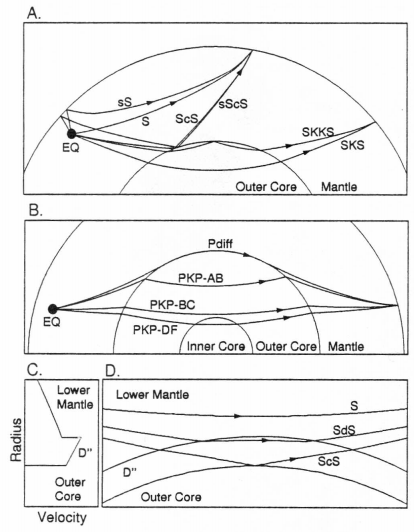
\includegraphics[width=0.85\textwidth]{wys_ray_path.png}
            
            \inc{wys_ray_path_cap.png}
        \end{center}
    \end{minipage}
    \begin{minipage}[c]{0.45\textwidth}
        \begin{itemize}
            \item P (primary, nyomás, longitudinális), S (secondary, nyírás, transzverzális) és felületi hullámok
            \item terjedési sebességük függ: közeg rugalmas tulajdonságai, sűrűség (hőméréklet)
            \item P és S hullámok egymásba alakulhatnak fázishatároknál
        \end{itemize}
        \cite{wysession}
    \end{minipage}
\end{frame}


\begin{frame}{Szeizmológiai alapok}
    \begin{figp}{\inc{helf_ray_paths.png}}{\cite{helffrich}}{0.45}{0.525}
        \begin{itemize}
            \item szeizmikus hullámok 3 módon hordoznak információt:
            \begin{itemize}
                \item hullám terjedési ideje (ismert terjedési útvonal $\rar$ átlagos útvonal menti sebesség- vagy sebesség anomália)
                \item másodlagos beérkezések $\lar$ lemez jelenléte (P $\rar$ S és S $\rar$ P diszkontinuitás a kőzet rugalmas tulajdonságaiban)
                \item frekv. függő hatások; $\lambda_i = n \cdot d_i$, $\lambda_i$-k felerősödnek/gyengülnek
            \end{itemize}
            \item szeizmológiai vizsgálatok $\rar$ sebesség (anomália) a lemez egy adott részén vagy rétegvastagság
            \item ásványtanból számított rugalmas hullám sebességek $\leftrightarrow$ szeizmikus hullám sebességek
        \end{itemize}
    \end{figp}
\end{frame}
